\chapter{Explanations of Important Terms And
Concepts}\label{explanations-of-important-terms-and-concepts}

\section{Autotrophs and Heterotrophs}\label{autotrophs-and-heterotrophs}

An \href{https://en.wikipedia.org/wiki/Autotroph}{autotroph}
(``self-feeding'', from the Greek autos ``self'' and trophe
``nourishing'') or producer, is an organism that produces complex
organic compounds (such as carbohydrates, fats, and proteins) from
simple substances present in its surroundings, generally using energy
from light (photosynthesis) or inorganic chemical reactions
(chemosynthesis). They are the producers in a food chain, such as plants
on land or algae in water. Autotrophs can reduce carbon dioxide to make
organic compounds for biosynthesis and also create a store of chemical
energy. Most autotrophs use water as the reducing agent, but some can
use other hydrogen compounds such as hydrogen sulfide.

Autotrophs can be photoautotrophs or chemoautotrophs. Phototrophs use
light as an energy source, while chemotrophs use electron donors as a
source of energy, whether from organic or inorganic sources; however, in
the case of autotrophs, these electron donors come from inorganic
chemical sources. Such chemotrophs are lithotrophs. Lithotrophs use
inorganic compounds, such as hydrogen sulfide, elemental sulfur,
ammonium and ferrous iron, as reducing agents for biosynthesis and
chemical energy storage. Photoautotrophs and lithoautotrophs use a
portion of the ATP produced during photosynthesis or the oxidation of
inorganic compounds to reduce NADP\textsuperscript{+} to NADPH to form organic compounds.

A \href{https://en.wikipedia.org/wiki/Heterotroph}{heterotroph} Greek
héteros = ``other'' plus trophe = ``nutrition'') is an organism that
ingests or absorbs organic carbon (rather than fix carbon from inorganic
sources such as carbon dioxide) in order to be able to produce energy
and synthesize compounds to maintain its life. Ninety-five percent or
more of all types of living organisms are heterotrophic, including all
animals and fungi and some bacteria and protists.

\href{https://en.wikipedia.org/wiki/Detritivore}{Detritivores} are
heterotrophs which obtain nutrients by consuming detritus (decomposing
plant and animal parts as well as feces). Saprotrophs (also called
lysotrophs) are chemoheterotrophs that use extracellular digestion in
processing decayed organic matter. It is a term most often associated
with fungi. The process is most often facilitated through the active
transport of such materials through endocytosis within the internal
mycelium and its constituent hyphae. 

\section{Biological Life Cycle}\label{biological-life-cycle}

A \href{https://en.wikipedia.org/wiki/Biological_life_cycle}{biological
life cycle} is a series of changes in form that an organism undergoes,
returning to the starting state. Transitions of form may involve growth,
asexual reproduction, or sexual reproduction. In some organisms,
different ``generations'' of the species succeed each other during the
life cycle. For plants and many algae, there are two multicellular
stages, and the life cycle is referred to as alternation of generations.
Life cycles that include sexual reproduction involve alternating haploid
(n) and diploid (2n) stages, i.e., a change of ploidy is involved. To
return from a diploid stage to a haploid stage, meiosis must occur. In
regard to changes of ploidy, there are 3 types of life cycles that we
will encounter in this course:

\begin{enumerate}
\def\labelenumi{\arabic{enumi}.}
\tightlist
\item
  \textbf{haplontic life cycle} (e.g.~in fungi): the haploid stage is
  multicellular and the diploid stage is a single cell, meiosis is
  ``zygotic''.
\item
  \textbf{diplontic life cycle} (e.g.~in animals): the diploid stage is
  multicellular and haploid gametes are formed, meiosis is ``gametic''.
\item
  \textbf{haplodiplontic life cycle} (e.g.~in plants): multicellular
  diploid (e.g.~the sporophyte in plants) and haploid stages (e.g.~the
  gametophyte in plants) occur, meiosis is ``sporic''.
\end{enumerate}

The cycles differ in when mitosis (growth) occurs. Zygotic meiosis and
gametic meiosis have one mitotic stage: mitosis occurs during the n
(haploid) phase in zygotic meiosis (e.g.~in fungi) and during the 2n
(diploid) phase in gametic meiosis (e.g.~in animals). Therefore, zygotic
and gametic meiosis are collectively termed haplobiontic (single mitotic
phase, not to be confused with haplontic). Sporic meiosis (e.g.~in
plants), on the other hand, has mitosis in two stages, both the diploid
and haploid stages, termed diplobiontic (not to be confused with
diplontic).

\section{Asexual and Sexual
Reproduction}\label{asexual-and-sexual-reproduction}

\href{https://en.wikipedia.org/wiki/Reproduction}{Reproduction} (or
procreation or breeding) is the biological process by which new
individual organisms -- ``offspring'' -- are produced from their
``parents''. Reproduction is a fundamental feature of all known life;
each individual organism exists as the result of reproduction. There are
two forms of reproduction: asexual and sexual.

Asexual reproduction is a process by which organisms create genetically
similar or identical copies of themselves without the contribution of
genetic material from another organism.

Sexual reproduction creates a new organism by combining the genetic
material of two organisms. Most animals and plants reproduce sexually.
Each of two parent organisms contributes half of the offspring's genetic
makeup by creating haploid gametes. Most organisms form two different
types of gametes. In these anisogamous species, the two sexes are
referred to as male (producing sperm or microspores) and female
(producing ova or megaspores). In isogamous species, the gametes are
similar or identical in form (isogametes). Because both gametes look
alike, they cannot be classified as ``male'' or ``female.'' Instead,
organisms undergoing isogamy are said to have different mating types,
most commonly noted as ``+'' and ``−'' strains. Sexual reproduction in
fungi differs in many aspects from sexual reproduction in animals or
plants. Sexually compatible fungi combine by fusing their hyphae
together. Many fungi go through a dikaryotic stage, in which the nuclei
inherited from the two parents do not combine immediately after cell
fusion, but remain separate in the hyphal cells. Sexually reproducing
organisms have different sets of genes for every trait (called alleles).
Offspring inherit one allele for each trait from each parent. Thus,
offspring have a combination of the parents' genes.

\section{Multicellularity}\label{multicellularity}

\href{https://en.wikipedia.org/wiki/Multicellular_organism}{Multicellular
organisms} are organisms that consist of more than one cell, in contrast
to unicellular organisms. Multicellularity allows an organism to exceed
the size limits normally imposed by diffusion: single cells with
increased size have a decreased surface-to-volume ratio and have
difficulty absorbing sufficient nutrients and transporting them
throughout the cell. Multicellular organisms thus have the competitive
advantages of an increase in size without its limitations. They can have
longer lifespans as they can continue living when individual cells die.
Multicellularity also permits increasing complexity by allowing
differentiation of cell types within one organism. One hypothesis for
the origin of multicellularity is that a group of function-specific
cells aggregated into a slug-like mass, which moved as a multicellular
unit. This is essentially what slime molds do. Another hypothesis is
that a primitive cell underwent nucleus division, thereby becoming a
coenocyte. A membrane would then form around each nucleus (and the
cellular space and organelles occupied in the space), thereby resulting
in a group of connected cells in one organism (this mechanism is
observable in the fruit fly Drosophila). A third hypothesis is that as a
unicellular organism divided, the daughter cells failed to separate,
resulting in a conglomeration of identical cells in one organism, which
could later develop specialized tissues. This is what plant and animal
embryos do as well as colonial choanoflagellates.

\section{Species}\label{species}

In biology, a \href{https://en.wikipedia.org/wiki/Species}{species} is
the basic unit of biological classification and a taxonomic rank, as
well as a unit of biodiversity. Scientists and others need a species
definition which allows them to work, regardless of the theoretical
difficulties. If as Linnaeus thought, species were fixed, there would be
no problem, but evolutionary processes cause species to change
continually, and to grade into one another. A species is often defined
as the largest group of organisms in which two individuals can produce
fertile offspring, typically by sexual reproduction. While this
definition is often adequate, when looked at more closely it is
problematic. For example, with hybridization, in a species complex of
hundreds of similar microspecies, or in a ring species, the boundaries
between closely related species become unclear. Among organisms that
reproduce only asexually, the concept of a reproductive species breaks
down, and each clone is potentially a microspecies. Problems also arise
when dealing with fossils, since reproduction cannot be examined. Other
ways of defining species include their karyotype, DNA sequence,
morphology, behavior or ecological niche.

All species are given a two-part name, a ``binomial'' (see below). The
first part of a binomial is the genus to which the species belongs. The
second part is called the specific name or the specific epithet (in
botanical nomenclature, also sometimes in zoological nomenclature). For
example, \emph{Boa constrictor} is one of four species of the \emph{Boa} genus.

Species were seen from the time of Aristotle until the 18th century as
fixed kinds that could be arranged in a hierarchy, the great chain of
being. In the 19th century, biologists grasped that species could evolve
given sufficient time. Charles Darwin's 1859 book \href{https://en.wikipedia.org/wiki/On_the_Origin_of_Species}{On The Origin of Species}
explained how species could arise by natural selection. That
understanding was greatly extended in the 20th century through genetics
and population ecology. Genetic variability arises from mutations and
recombination, while organisms themselves are mobile, leading to
geographical isolation and \href{https://en.wikipedia.org/wiki/Genetic_drift}{genetic drift} with varying selection
pressures. Genes can sometimes be exchanged between species by
\href{https://en.wikipedia.org/wiki/Horizontal_gene_transfer}{horizontal gene transfer}; new species can arise rapidly through
\href{https://en.wikipedia.org/wiki/Hybrid_(biology)}{hybridization} and \href{https://en.wikipedia.org/wiki/Polyploid}{polyploidy}; and species may become extinct for a
variety of reasons. Viruses are a special case, driven by a balance of
mutation and selection, and can be treated as quasispecies.

As a practical matter, species concepts may be used to define species
that are then used to measure biodiversity, though whether this is a
good measure is disputed, as other measures are possible.

The commonly used names for kinds of organisms are often ambiguous:
``cat'' could mean the domestic cat, \emph{Felis catus}, or the cat family,
Felidae. Another problem with common names is that they often vary from
place to place, so that puma, cougar, catamount, panther, painter and
mountain lion all mean \emph{Puma concolor} in various parts of America, while
``panther'' may also mean the jaguar (\emph{Panthera onca}) of Latin America or
the leopard (\emph{Panthera pardus}) of Africa and Asia. In contrast, the
scientific names of species are chosen to be unique and universal; they
are in two parts used together: the genus as in \emph{Puma}, and the specific
epithet as in \emph{concolor}. A species is given a taxonomic name when a type
specimen is described formally, in a publication that assigns it a
unique scientific name. The description typically provides means for
identifying the new species, differentiating it from other previously
described and related or confusable species and provides a validly
published name (in botany) or an available name (in zoology) when the
paper is accepted for publication. The type material is usually held in
a permanent repository, often the research collection of a major museum
or university, that allows independent verification and the means to
compare specimens. Describers of new species are asked to choose names
that, in the words of the International Code of Zoological Nomenclature,
are ``appropriate, compact, euphonious, memorable, and do not cause
offence.''

Biologists and taxonomists have made many attempts to define species,
beginning from morphology and moving towards genetics. Early taxonomists
such as Linnaeus had no option but to describe what they saw: this was
later formalized as the typological or morphological species concept.
Mayr emphasized reproductive isolation, but this, like other species
concepts, is hard or even impossible to test. Many of the concepts are
quite similar or overlap, so they are not easy to count.

The evolutionary process by which biological populations evolve to
become distinct or reproductively isolated as species is called
\href{https://en.wikipedia.org/wiki/Speciation}{speciation}. Charles Darwin described the role of natural selection in
speciation in his 1859 book On The Origin of Species. Speciation depends on
a measure of \href{https://en.wikipedia.org/wiki/Reproductive_isolation}{reproductive isolation}, a reduced gene flow. This occurs
most easily in \href{https://en.wikipedia.org/wiki/Allopatric_speciation}{allopatric speciation}, where populations are separated
geographically and can diverge gradually as mutations accumulate.
Reproductive isolation is threatened by hybridization, but this can be
selected against once a pair of populations have incompatible alleles of
the same gene, as described in the Bateson--Dobzhansky--Muller model. A
different mechanism, phyletic speciation, involves one lineage gradually
changing over time into a new and distinct form, without increasing the
number of resultant species.

A species is extinct when the last individual of that species dies, but
it may be functionally extinct well before that moment. It is estimated
that over 99 percent of all species that ever lived on Earth, some five
billion species, are now extinct. Some of these were in mass extinctions
such as those at the ends of the Permian, Triassic and Cretaceous
periods. Mass extinctions had a variety of causes including volcanic
activity, climate change, and changes in oceanic and atmospheric
chemistry, and they in turn had major effects on Earth's ecology,
atmosphere, land surface, and waters. Another form of extinction is
through the assimilation of one species by another through
hybridization. 

\section{Evolution}\label{evolution}

\href{https://en.wikipedia.org/wiki/Evolution}{Evolution} is change in
the heritable characteristics of biological populations over successive
generations. Evolutionary processes give rise to biodiversity at every
level of biological organization, including the levels of species,
individual organisms, and molecules.

Repeated formation of new species (speciation), change within species
(anagenesis), and loss of species (extinction) throughout the
evolutionary history of life on Earth are demonstrated by shared sets of
morphological and biochemical traits, including shared DNA sequences.
These shared traits are more similar among species that share a more
recent common ancestor, and can be used to reconstruct a biological
``tree of life'' based on evolutionary relationships (phylogenetics),
using both existing species and fossils. The fossil record includes a
progression from early biogenic graphite, to microbial mat fossils, to
fossilized multicellular organisms. Existing patterns of biodiversity
have been shaped both by speciation and by extinction.

\href{https://en.wikipedia.org/wiki/Charles_Darwin}{Charles Darwin}
developed his theory of ``natural selection'' from 1838 onwards and was
writing up his ``big book'' on the subject when
\href{https://en.wikipedia.org/wiki/Alfred_Russel_Wallace}{Alfred Russel
Wallace} sent him a version of virtually the same theory in 1858. Their
separate papers were presented together at an 1858 meeting of the
Linnaean Society of London. At the end of 1859, Darwin's book ``On the
Origin of Species'' explained natural selection in detail and in a way,
that led to an increasingly wide acceptance of Darwin's concepts of
evolution at the expense of alternative theories.

According to \href{https://en.wikipedia.org/wiki/Ernst_Mayr}{Ernst
Mayr}, Darwin's theory actually consists of a number of different
theories that can be best understood when they are clearly distinguished
from each other. Mayr distinguished five independent theories:

\begin{enumerate}
\def\labelenumi{\arabic{enumi}.}
\tightlist
\item
  The non-constancy of species (the basic theory of evolution)
\item
  The descent of all organisms from common ancestors (branching
  evolution)
\item
  The gradualness of evolution (no saltations, no discontinuities)
\item
  The multiplication of species (the origin of diversity)
\item
  Natural selection
\end{enumerate}

The first and second theories were widely accepted by biologists rather
quickly following Darwin's publication. The other three theories were
not widely accepted until the arrival of the so-called modern synthesis
in the 20th century (see below).

Evolution by
\href{https://en.wikipedia.org/wiki/Natural_selection}{natural
selection} is a process demonstrated by the observation that more
offspring are produced than can possibly survive, along with three facts
about populations: 1) traits vary among individuals with respect to
morphology, physiology, and behavior (phenotypic variation), 2)
different traits confer different rates of survival and reproduction
(differential fitness), and 3) traits can be passed from generation to
generation (heritability of fitness). Thus, in successive generations
members of a population are replaced by progeny of parents better
adapted to survive and reproduce in the biophysical environment in which
natural selection takes place.

The four most widely recognized evolutionary processes are natural
selection (including sexual selection),
\href{https://en.wikipedia.org/wiki/Genetic_drift}{genetic drift},
\href{https://en.wikipedia.org/wiki/Mutation}{mutation} and
\href{https://en.wikipedia.org/wiki/Gene_flow}{gene migration} due to
genetic admixture. Natural selection and genetic drift sort variation;
mutation and gene migration create variation.

The mechanisms of reproductive heritability and the origin of new traits
remained a mystery. Towards this end, Darwin developed his provisional
theory of pangenesis. In 1865, \href{https://en.wikipedia.org/wiki/Gregor_Mendel}{Gregor Mendel} reported that traits were
inherited in a predictable manner through the independent assortment and
segregation of elements (later known as genes). Mendel's laws of
inheritance eventually supplanted most of Darwin's pangenesis theory.
\href{https://en.wikipedia.org/wiki/August_Weismann}{August Weismann} made the important distinction between germ cells that
give rise to gametes (such as sperm and egg cells) and the somatic cells
of the body, demonstrating that heredity passes through the germ line
only. \href{https://en.wikipedia.org/wiki/Hugo_de_Vries}{Hugo de Vries} connected Darwin's pangenesis theory to Weismann's
germ/soma cell distinction and proposed that Darwin's pangenes were
concentrated in the cell nucleus and when expressed they could move into
the cytoplasm to change the cells structure. de Vries was also one of
the researchers who made Mendel's work well-known, believing that
Mendelian traits corresponded to the transfer of heritable variations
along the germline. de Vries developed a mutation theory to explain how
new variants originate. This led to a temporary rift between those who
accepted Darwinian evolution and biometricians who allied with de Vries.
In the 1930s, pioneers in the field of population genetics, such as
\href{}{Ronald Fisher}, \href{https://en.wikipedia.org/wiki/Sewall_Wright}{Sewall Wright} and \href{https://en.wikipedia.org/wiki/J._B._S._Haldane}{J. B. S. Haldane} set the foundations of
evolution onto a robust statistical philosophy. The false contradiction
between Darwin's theory, genetic mutations, and Mendelian inheritance
was thus reconciled.

In the 1920s and 1930s the so-called
\href{https://en.wikipedia.org/wiki/Modern_synthesis_(20th_century)}{modern
synthesis} connected natural selection and population genetics, based on
Mendelian inheritance, into a unified theory that applied generally to
any branch of biology. The modern synthesis explained patterns observed
across species in populations, through fossil transitions in
paleontology, and complex cellular mechanisms in developmental biology.
The publication of the structure of
\href{https://en.wikipedia.org/wiki/DNA}{DNA} by
\href{https://en.wikipedia.org/wiki/James_Watson}{James Watson} and
\href{https://en.wikipedia.org/wiki/Francis_Crick}{Francis Crick} in
1953 demonstrated a physical mechanism for inheritance. Molecular
biology improved our understanding of the relationship between genotype
and phenotype. Advancements were also made in phylogenetic systematics,
mapping the transition of traits into a comparative and testable
framework through the publication and use of evolutionary trees. In
1973, evolutionary biologist
\href{https://en.wikipedia.org/wiki/Theodosius_Dobzhansky}{Theodosius
Dobzhansky} penned that ``nothing in biology makes sense except in the
light of evolution,'' because it has brought to light the relations of
what first seemed disjointed facts in natural history into a coherent
explanatory body of knowledge that describes and predicts many
observable facts about life on this planet.

All life on Earth shares a common ancestor known as the
\href{https://en.wikipedia.org/wiki/Last_universal_common_ancestor}{last
universal common ancestor} (LUCA), which lived approximately 3.5--3.8
billion years ago.

In terms of practical application, an understanding of evolution has
been instrumental to developments in numerous scientific and industrial
fields, including agriculture, human and veterinary medicine, and the
life sciences in general. Discoveries in evolutionary biology have made
a significant impact not just in the traditional branches of biology but
also in other academic disciplines, including biological anthropology,
and evolutionary psychology.

\section{Phylum}\label{phylum}

In biology, a \href{https://en.wikipedia.org/wiki/Phylum}{phylum}
(plural: phyla) is a level of classification or taxonomic rank below
Kingdom and above Class. Traditionally, in botany the term division has
been used instead of phylum. Depending on definitions, the animal
kingdom Animalia or Metazoa contains approximately 33 phyla, the plant
kingdom Plantae contains about 14, and the fungus kingdom Fungi contains
about 8 phyla. Current research in phylogenetics (see below) is
uncovering the relationships between phyla, which are contained in
larger clades, like Ecdysozoa and Embryophyta.

The term phylum was coined by \href{https://en.wikipedia.org/wiki/Ernst_Haeckel}{Ernst Haeckel} from the Greek phylon,
``race, stock,'' related to phyle, ``tribe, clan.'' In plant taxonomy,
\href{https://en.wikipedia.org/wiki/August_W._Eichler}{August W. Eichler} (1883) classified plants into five groups named
divisions, a term that remains in use today for groups of plants, algae
and fungi.

Informally, phyla can be thought of as groupings of organisms based on
general specialization of body plan. At its most basic, a phylum can be
defined in two ways: as a group of organisms with a certain degree of
morphological or developmental similarity (the phenetic definition), or
a group of organisms with a certain degree of evolutionary relatedness
(the phylogenetic definition).

\section{Phylogenetics}\label{phylogenetics}

In biology,
\href{https://en.wikipedia.org/wiki/Phylogenetics}{phylogenetics}
(Greek: phylé, phylon = tribe, clan, race + genetikós = origin, source,
birth) is the study of the evolutionary history and relationships among
individuals or groups of organisms (e.g.~species, or populations). These
relationships are discovered through phylogenetic inference methods that
evaluate observed heritable traits, such as DNA sequences or morphology
under a model of evolution of these traits. The result of these analyses
is a phylogeny (also known as a phylogenetic tree) -- a diagrammatic
hypothesis about the history of the evolutionary relationships of a
group of organisms. The tips of a phylogenetic tree can be living
organisms or fossils, and represent the ``end'', or the present, in an
evolutionary lineage. Phylogenetic analyses have become central to
understanding biodiversity, evolution, ecology, and genomes.

Taxonomy is the identification, naming and classification of organisms.
It is usually richly informed by phylogenetics, but remains a
methodologically and logically distinct discipline. The degree to which
taxonomies depend on phylogenies (or classification depends on
evolutionary development) differs depending on the school of taxonomy:
phenetics (Greek: phainein - to appear) ignores phylogeny altogether and
attempts to classify organisms based on overall similarity, usually in
morphology or other observable traits, regardless of their phylogeny or
evolutionary relation; cladistics (phylogenetic systematics) tries to
reproduce phylogeny in its classification without loss of information;
evolutionary taxonomy tries to find a compromise between them.  

\section{Taxonomy}\label{taxonomy}

\href{https://en.wikipedia.org/wiki/Taxonomy_(biology)}{Taxonomy} (from
Ancient Greek taxis, meaning `arrangement', and nomia, meaning `method')
is the science of defining and naming groups of biological organisms on
the basis of shared characteristics. Organisms are grouped together into
taxa (singular: taxon) and these groups are given a taxonomic rank;
groups of a given rank can be aggregated to form a super-group of higher
rank, thus creating a taxonomic hierarchy. The principal ranks in modern
use are domain, kingdom, phylum (division is sometimes used in botany in
place of phylum), class, order, family, genus and species. The Swedish
botanist \href{https://en.wikipedia.org/wiki/Carl_Linnaeus}{Carl Linnaeus} (1707--1778) is regarded as the father of taxonomy, as he
developed a system known as Linnaean taxonomy for categorization of
organisms and binomial nomenclature for naming organisms.

With the advent of such fields of study as phylogenetics, cladistics,
and systematics, the Linnaean system has progressed to a system of
modern biological classification based on the evolutionary relationships
between organisms, both living and extinct.

Linnaeus ushered in a new era of taxonomy. With his major works
Systema Naturae 1st Edition in 1735, Species Plantarum in 1753, and
Systema Naturae 10th Edition, he revolutionized modern taxonomy. His
works implemented a standardized binomial naming system for animal and
plant species, which proved to be an elegant solution to a chaotic and
disorganized taxonomic literature. He not only introduced the standard
of class, order, genus, and species, but also made it possible to
identify plants and animals from his book, by using the smaller parts of
the flower. Thus, the Linnaean system was born, and is still used in
essentially the same way today as it was in the 18th century. Currently,
plant and animal taxonomists regard Linnaeus' work as the ``starting
point'' for valid names (at 1753 and 1758 respectively). Names published
before these dates are referred to as ``pre-Linnaean'', and not
considered valid (with the exception of spiders published in Svenska
Spindlar). Even taxonomic names published by Linnaeus himself before
these dates are considered pre-Linnaean.

Whereas Linnaeus classified for ease of identification, the idea of the
Linnaean taxonomy as translating into a sort of dendrogram of the
Animal- and Plant Kingdoms was formulated toward the end of the 18th
century, well before On the Origin of Species was published. Among early
works exploring the idea of a transmutation of species were Erasmus \href{https://en.wikipedia.org/wiki/Erasmus_Darwin}{Darwin's} 1796 Zoönomia and Jean-Baptiste \href{https://en.wikipedia.org/wiki/Jean-Baptiste_Lamarck}{Lamarck's} Philosophie
Zoologique of 1809. The idea was popularized in the Anglophone world by
the speculative but widely read \href{https://en.wikipedia.org/wiki/Vestiges_of_the_Natural_History_of_Creation}{Vestiges of the Natural History of
Creation}, published anonymously by Robert \href{https://en.wikipedia.org/wiki/Robert_Chambers_(publisher,_born_1802)}{Chambers} in 1844.

With Darwin's theory, a general acceptance quickly appeared that a
classification should reflect the Darwinian principle of common descent.
Tree of life representations became popular in scientific works, with
known fossil groups incorporated. One of the first modern groups tied to
fossil ancestors was birds. Using the then newly discovered fossils of
Archaeopteryx and Hesperornis, Thomas Henry Huxley pronounced that they
had evolved from dinosaurs, a group formally named by Richard \href{https://en.wikipedia.org/wiki/Richard_Owen}{Owen} in
1842. The resulting description, that of dinosaurs ``giving rise to'' or
being ``the ancestors of'' birds, is the essential hallmark of
evolutionary taxonomic thinking. As more and more fossil groups were
found and recognized in the late 19th and early 20th centuries,
paleontologists worked to understand the history of animals through the
ages by linking together known groups. With the modern evolutionary
synthesis of the early 1940s, an essentially modern understanding of the
evolution of the major groups was in place.

The cladistic method has emerged since the 1960s. In 1958, \href{https://en.wikipedia.org/wiki/Julian_Huxley}{Julian Huxley}
used the term clade. Later, in 1960, Cain and Harrison introduced the
term cladistic. The salient feature is arranging taxa in a hierarchical
evolutionary tree, ignoring ranks. A taxon is called monophyletic, if it
includes all the descendants of an ancestral form. Groups that have
descendant groups removed from them (e.g.~dinosaurs, with birds as
offspring group) are termed paraphyletic, while groups representing more
than one branch from the tree of life are called polyphyletic. The
International Code of Phylogenetic Nomenclature or PhyloCode is intended
to regulate the formal naming of clades. Linnaean ranks will be optional
under the PhyloCode, which is intended to coexist with the current,
rank-based codes.

Well before Linnaeus, plants and animals were considered separate
Kingdoms. Linnaeus used this as the top rank, dividing the physical
world into the plant, animal and mineral kingdoms. As advances in
microscopy made classification of microorganisms possible, the number of
kingdoms increased, five and six-kingdom systems being the most common.

Domains are a relatively new grouping. First proposed in 1977,
\href{https://en.wikipedia.org/wiki/Carl_Woese}{Carl Woese's}
three-domain system was not generally accepted until later. One main
characteristic of the three-domain method is the separation of \href{https://en.wikipedia.org/wiki/Archaea}{Archaea}
and \href{https://en.wikipedia.org/wiki/Bacteria}{Bacteria}, previously grouped into the single kingdom Bacteria (a
kingdom also sometimes called Monera), with the \href{https://en.wikipedia.org/wiki/Eukaryote}{Eukaryota} for all
organisms whose cells contain a nucleus.

\begin{figure}

{\centering 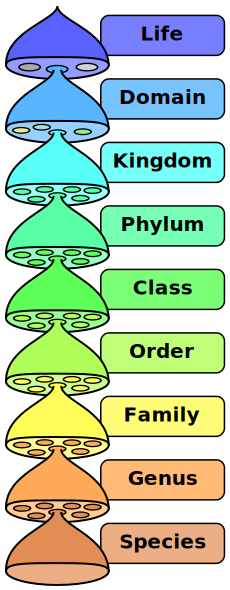
\includegraphics[width=0.7\linewidth]{./figures/appendix1/biological_classification}

}

\caption{\href{https://commons.wikimedia.org/wiki/File:Biological_classification_L_Pengo_vflip.svg}{Biological
classification.}}\label{fig:classification}
\end{figure}

Biological classification is a critical component of the taxonomic
process. As a result, it informs the user as to what the relatives of
the taxon are hypothesized to be. Biological classification uses
taxonomic ranks, including among others (in order from most inclusive to
least inclusive): Domain, Kingdom, Phylum, Class, Order, Family, Genus,
and Species

The ``definition'' of a taxon is encapsulated by its description or its
diagnosis or by both combined. There are no set rules governing the
definition of taxa, but the naming and publication of new taxa is
governed by sets of rules. In zoology, the nomenclature for the more
commonly used ranks (superfamily to subspecies), is regulated by the
International Code of Zoological Nomenclature (ICZN Code). In the fields
of botany, phycology, and mycology, the naming of taxa is governed by
the International Code of Nomenclature for algae, fungi, and plants
(ICN).

The initial description of a taxon involves five main requirements:

\begin{enumerate}
\def\labelenumi{\arabic{enumi}.}
\tightlist
\item
  The taxon must be given a name based on the 26 letters of the Latin
  alphabet (a binomial for new species, or uninomial for other ranks).
\item
  The name must be unique (i.e.~not a homonym).
\item
  The description must be based on at least one name-bearing type
  specimen.
\item
  It should include statements about appropriate attributes either to
  describe (define) the taxon or to differentiate it from other taxa
  (the diagnosis, ICZN Code, Article 13.1.1, ICN, Article 38). Both
  codes deliberately separate defining the content of a taxon (its
  circumscription) from defining its name.
\item
  These first four requirements must be published in a work that is
  obtainable in numerous identical copies, as a permanent scientific
  record.
\end{enumerate}

However, often much more information is included, like the geographic
range of the taxon, ecological notes, chemistry, behavior, etc. How
researchers arrive at their taxa varies: depending on the available
data, and resources, methods vary from simple quantitative or
qualitative comparisons of striking features, to elaborate computer
analyses of large amounts of DNA sequence data.

An ``authority'' may be placed after a scientific name. The authority is
the name of the scientist or scientists who first validly published the
name. For example, in 1758 Linnaeus gave the Asian elephant the
scientific name Elephas maximus, so the name is sometimes written as
``Elephas maximus Linnaeus, 1758''. The names of authors are frequently
abbreviated: the abbreviation L., for Linnaeus, is commonly used. In
botany, there is, in fact, a regulated list of standard abbreviations
(see list of botanists by author abbreviation). The system for assigning
authorities differs slightly between botany and zoology. However, it is
standard that if a species' name or placement has been changed since the
original description, the original authority's name is placed in
parentheses.

\begin{figure}

{\centering 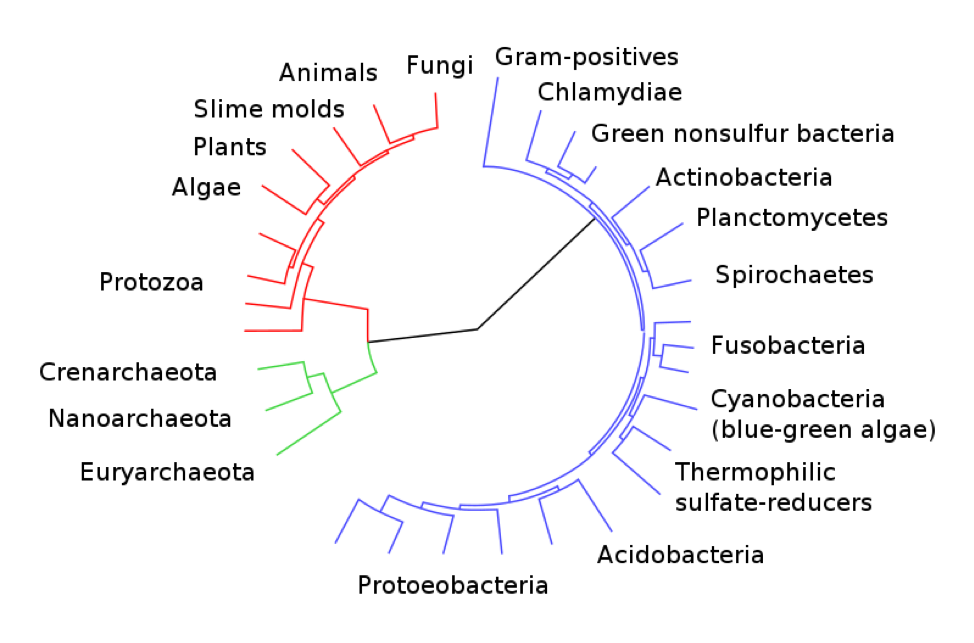
\includegraphics[width=0.7\linewidth]{./figures/appendix1/tree_of_life}

}

\caption{\href{https://commons.wikimedia.org/wiki/File:CollapsedtreeLabels-simplified.svg}{The
tree of life.}}\label{fig:tree}
\end{figure}

\section{Cladistics}\label{cladistics}

\href{https://en.wikipedia.org/wiki/Cladistics}{Cladistics} (from Greek
klados, i.e., ``branch'') is an approach to biological classification in
which organisms are categorized based on shared derived characteristics
that can be traced to a group's most recent common ancestor and are not
present in more distant ancestors. Therefore, members of a group are
assumed to share a common history and are considered to be closely
related.

The original methods used in cladistic analysis and the school of
taxonomy derived from the work of the German entomologist \href{https://en.wikipedia.org/wiki/Willi_Hennig}{Willi Hennig},
who referred to it as phylogenetic systematics (also the title of his
1966 book); the terms ``cladistics'' and ``clade'' were popularized by
other researchers. Cladistics in the original sense refers to a
particular set of methods used in phylogenetic analysis, although it is
now sometimes used to refer to the whole field.

The following terms, coined by Hennig, are used to identify shared or
distinct character states among groups of organisms:

\begin{itemize}
\item
  A \textbf{plesiomorphy} (``close form'') or ancestral state is a
  character state that a taxon has retained from its ancestors. When two
  or more taxa that are not nested within each other share a
  plesiomorphy, it is a symplesiomorphy (from syn-, ``together'').
  Symplesiomorphies do not mean that the taxa that exhibit that
  character state are necessarily closely related. For example, Reptilia
  is traditionally characterized by (among other things) being
  cold-blooded (i.e., not maintaining a constant high body temperature),
  whereas birds are warm-blooded. Since cold-bloodedness is a
  plesiomorphy, inherited from the common ancestor of traditional
  reptiles and birds, and thus a symplesiomorphy of turtles, snakes and
  crocodiles (among others), it does not mean that turtles, snakes and
  crocodiles form a clade that excludes the birds.
\item
  An \textbf{apomorphy} (``separate form'') or derived state is an
  innovation. It can thus be used to diagnose a clade -- or even to help
  define a clade name in phylogenetic nomenclature. Features that are
  derived in individual taxa (a single species or a group that is
  represented by a single terminal in a given phylogenetic analysis) are
  called autapomorphies (from auto-, ``self''). Autapomorphies express
  nothing about relationships among groups; clades are identified (or
  defined) by synapomorphies (from syn-, ``together''). For example, the
  possession of digits that are homologous with those of Homo sapiens is
  a synapomorphy within the vertebrates. The tetrapods can be singled
  out as consisting of the first vertebrate with such digits homologous
  to those of Homo sapiens together with all descendants of this
  vertebrate (an apomorphy-based phylogenetic definition). Importantly,
  snakes and other tetrapods that do not have digits are nonetheless
  tetrapods: other characters, such as amniotic eggs and diapsid skulls,
  indicate that they descended from ancestors that possessed digits
  which are homologous with ours.
\item
  A \textbf{character state} is homoplastic or ``an instance of
  homoplasy'' if it is shared by two or more organisms but is absent
  from their common ancestor or from a later ancestor in the lineage
  leading to one of the organisms. It is therefore inferred to have
  evolved by convergence or reversal. Both mammals and birds are able to
  maintain a high constant body temperature (i.e., they are
  warm-blooded). However, the accepted cladogram explaining their
  significant features indicates that their common ancestor is in a
  group lacking this character state, so the state must have evolved
  independently in the two clades. Warm-bloodedness is separately a
  synapomorphy of mammals (or a larger clade) and of birds (or a larger
  clade), but it is not a synapomorphy of any group including both these
  clades. Hennig's Auxiliary Principle states that shared character
  states should be considered evidence of grouping unless they are
  contradicted by the weight of other evidence; thus, homoplasy of some
  feature among members of a group may only be inferred after a
  phylogenetic hypothesis for that group has been established.
\end{itemize}

The terms plesiomorphy and apomorphy are relative; their application
depends on the position of a group within a tree. For example, when
trying to decide whether the tetrapods form a clade, an important
question is whether having four limbs is a synapomorphy of the earliest
taxa to be included within Tetrapoda: did all the earliest members of
the Tetrapoda inherit four limbs from a common ancestor, whereas all
other vertebrates did not, or at least not homologously? By contrast,
for a group within the tetrapods, such as birds, having four limbs is a
plesiomorphy. Using these two terms allows a greater precision in the
discussion of homology, in particular allowing clear expression of the
hierarchical relationships among different homologous features.

It can be difficult to decide whether a character state is in fact the
same and thus can be classified as a synapomorphy, which may identify a
monophyletic group, or whether it only appears to be the same and is
thus a homoplasy, which cannot identify such a group. There is a danger
of circular reasoning: assumptions about the shape of a phylogenetic
tree are used to justify decisions about character states, which are
then used as evidence for the shape of the tree. Phylogenetics uses
various forms of parsimony to decide such questions; the conclusions
reached often depend on the dataset and the methods. Such is the nature
of empirical science, and for this reason, most cladists refer to their
cladograms as hypotheses of relationship. Cladograms that are supported
by a large number and variety of different kinds of characters are
viewed as more robust than those based on more limited evidence.

A \href{https://en.wikipedia.org/wiki/Monophyly}{monophyletic} group is
a group of organisms that forms a clade, which consists of all the
descendants of a common ancestor. Monophyletic groups are typically
characterized by shared derived characteristics (synapomorphies), which
distinguish organisms in the clade from other organisms. The arrangement
of the members of a monophyletic group is called a monophyly.

A group is \href{https://en.wikipedia.org/wiki/Paraphyly}{paraphyletic}
if it consists of the group's last common ancestor and all descendants
of that ancestor excluding a few---typically only one or
two---monophyletic subgroups. The group is said to be paraphyletic with
respect to the excluded subgroups. The arrangement of the members of a
paraphyletic group is called a paraphyly.

A \href{https://en.wikipedia.org/wiki/Polyphyly}{polyphyletic} (Greek
for ``of many races'') group is a set of organisms, or other evolving
elements, that have been grouped together but do not share an immediate
common ancestor. The term is often applied to groups that share
characteristics that appear to be similar but have not been inherited
from common ancestors; these characteristics are known as homoplasies,
and the development and phenomenon of homoplasies is known as convergent
evolution. The arrangement of the members of a polyphyletic group is
called a polyphyly.

\begin{figure}

{\centering 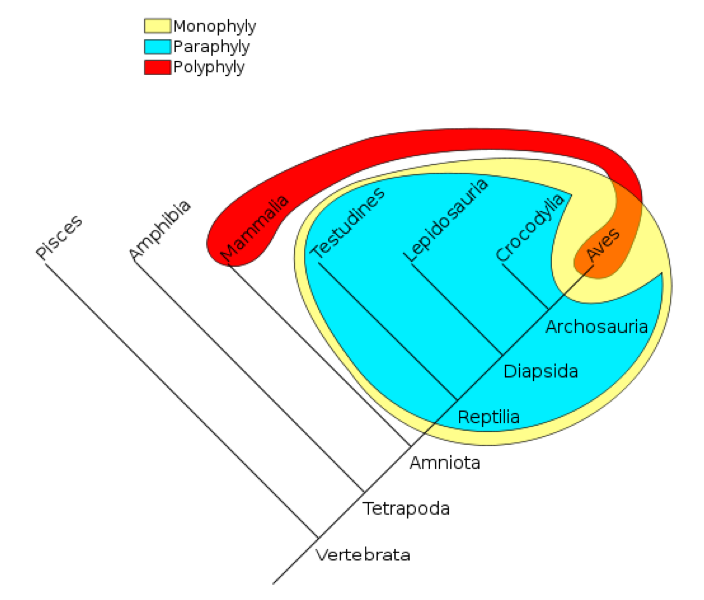
\includegraphics[width=0.7\linewidth]{./figures/appendix1/phylogenetic_groups}

}

\caption{\href{https://commons.wikimedia.org/wiki/File:Phylogenetic-Groups.svg}{Phylogenetic
groups.}}\label{fig:phylogeny}
\end{figure}

\section{Animal Clades}\label{animal-clades}

\section{Non-bilaterian Animals}\label{non-bilaterian-animals}

Several \href{https://en.wikipedia.org/wiki/Animal}{animal} phyla are
recognized for their lack of bilateral symmetry, and are thought to have
diverged from other animals early in evolution. Among these, the sponges
(Porifera) were long thought to have diverged first, representing the
oldest animal phylum. They lack the complex organization found in most
other phyla. Their cells are differentiated, but in most cases not
organized into distinct tissues. Sponges typically feed by drawing in
water through pores. However, a series of phylogenomic studies from
2008--2015 have found support for Ctenophora, or comb jellies, as the
basal lineage of animals. This result has been controversial, since it
would imply that sponges may not be so primitive, but may instead be
secondarily simplified. Other researchers have argued that the placement
of Ctenophora as the earliest-diverging animal phylum is a statistical
anomaly caused by the high rate of evolution in ctenophore genomes.

The Ctenophora and the sponges are unique among the animals in lacking
true hox genes. The presence of a Hox/Parahox gene in the Placozoa
suggests that either the Porifera or the Ctenophora are the most basal
animal clades.

\href{https://en.wikipedia.org/wiki/Hox_gene}{Hox genes} (a subset of
homeotic genes) are a group of related genes that control the body plan
of an embryo along the head-tail axis. In evolutionary developmental
biology, \href{https://en.wikipedia.org/wiki/Homeotic_gene}{homeotic genes} are genes which regulate the development of
anatomical structures in organisms. After the embryonic segments have
formed, the Hox proteins determine the type of appendages (e.g.~legs,
antennae, and wings in fruit flies) or the different types of vertebrae
(in humans) that will form on a segment. Hox proteins thus confer
segmental identity, but do not form the actual segments themselves.
Mutations in the Hox genes can result in body parts and limbs in the
wrong place along the body. The protein product of each Hox gene is a
transcription factor. Each Hox gene contains a well-conserved DNA
sequence known as the homeobox. Hox genes are thus a subset of the
homeobox transcription factor genes. In many animals, the organization
of the Hox genes in the chromosome is the same as the order of their
expression along the anterior-posterior axis of the developing animal,
and are thus said to display co-linearity.

Among the other phyla, the Ctenophora and the Cnidaria, which includes
sea anemones, corals, and jellyfish, are radially symmetric and have
digestive chambers with a single opening, which serves as both the mouth
and the anus. Both have distinct tissues, but they are not organized
into organs. There are only two main germ layers, the ectoderm and
endoderm, with only scattered cells between them. As such, these animals
are sometimes called diploblastic. The tiny placozoans are similar, but
they do not have a permanent digestive chamber.

The Myxozoa, microscopic parasites that were originally considered
Protozoa, are now believed to have evolved within Cnidaria.

\section{Bilaterian Animals}\label{bilaterian-animals}

The remaining animals form a monophyletic group called the \href{https://en.wikipedia.org/wiki/Bilateria}{Bilateria}.
For the most part, they are bilaterally symmetric, and often have a
specialized head with feeding and sensory organs. The body is
triploblastic, i.e.~all three germ layers are well-developed, and
tissues form distinct organs. The digestive chamber has two openings, a
mouth and an anus, and there is also an internal body cavity called a
coelom or pseudocoelom. There are exceptions to each of these
characteristics, however---for instance adult echinoderms are radially
symmetric, and certain parasitic worms have extremely simplified body
structures.

Genetic studies have considerably changed our understanding of the
relationships within the Bilateria. Most appear to belong to two major
lineages: the deuterostomes and the protostomes, the latter of which
includes the Ecdysozoa, and Lophotrochozoa. The Chaetognatha or arrow
worms have been traditionally classified as deuterostomes, though recent
molecular studies have identified this group as a basal protostome
lineage.

In addition, there are a few small groups of bilaterians with relatively
cryptic morphology whose relationships with other animals are not
well-established. For example, recent molecular studies have identified
\href{https://en.wikipedia.org/wiki/Acoelomorpha}{Acoelomorpha} and \href{https://en.wikipedia.org/wiki/Xenoturbella}{Xenoturbella} as forming a monophyletic group, but
studies disagree as to whether this group evolved from within
deuterostomes, or whether it represents the sister group to all other
bilaterian animals (\href{https://en.wikipedia.org/wiki/Nephrozoa}{Nephrozoa}). Other groups of uncertain affinity
include the \href{https://en.wikipedia.org/wiki/Dicyemida}{Rhombozoa} (also known as Dicyemida) and \href{https://en.wikipedia.org/wiki/Orthonectida}{Orthonectida}. One phyla, the Monoblastozoa,
was described by a scientist in 1892, but so far there have been no
evidence of its existence.

\section{Deuterostomes and
Protostomes}\label{deuterostomes-and-protostomes}

\href{https://en.wikipedia.org/wiki/Deuterostome}{Deuterostomes} differ
from \href{https://en.wikipedia.org/wiki/Protostome}{protostomes} in
several ways. Animals from both groups possess a complete digestive
tract. However, in protostomes, the first opening of the gut to appear
in embryological development (the archenteron) develops into the mouth,
with the anus forming secondarily. In deuterostomes the anus forms
first, with the mouth developing secondarily. In most protostomes, cells
simply fill in the interior of the gastrula to form the mesoderm, called
schizocoelous development, but in deuterostomes, it forms through
invagination of the endoderm, called enterocoelic pouching. Deuterostome
embryos undergo radial \href{https://en.wikipedia.org/wiki/Cleavage_(embryo)}{cleavage} during cell division, while protostomes
undergo spiral cleavage.

All this suggests the deuterostomes and protostomes are separate,
monophyletic lineages. The main phyla of deuterostomes are the
Echinodermata and Chordata. The former are radially symmetric and
exclusively marine, such as starfish, sea urchins, and sea cucumbers.
The latter are dominated by the vertebrates, animals with backbones.
These include fish, amphibians, reptiles, birds, and mammals.

In addition to these, the deuterostomes also include the Hemichordata,
or acorn worms, which are thought to be closely related to Echinodermata
forming a group known as Ambulacraria. Although they are not especially
prominent today, the important fossil graptolites may belong to this
group.

\section{Ecdysozoa}\label{ecdysozoa}

The \href{https://en.wikipedia.org/wiki/Ecdysozoa}{Ecdysozoa} are
protostomes, named after the common trait of growth by moulting or
ecdysis. The largest animal phylum belongs here, the Arthropoda,
including insects, spiders, crabs, and their kin. All these organisms
have a body divided into repeating segments, typically with paired
appendages. Two smaller phyla, the \href{https://en.wikipedia.org/wiki/Onychophora}{Onychophora} and \href{https://en.wikipedia.org/wiki/Tardigrade}{Tardigrada}, are close
relatives of the arthropods and share these traits. The ecdysozoans also
include the Nematoda or roundworms, perhaps the second largest animal
phylum. Roundworms are typically microscopic, and occur in nearly every
environment where there is water. A number are important parasites.
Smaller phyla related to them are the \href{https://en.wikipedia.org/wiki/Nematomorpha}{Nematomorpha} or horsehair worms,
and the \href{https://en.wikipedia.org/wiki/Kinorhyncha}{Kinorhyncha}, \href{https://en.wikipedia.org/wiki/Priapulida}{Priapulida}, and \href{https://en.wikipedia.org/wiki/Loricifera}{Loricifera}. These groups have a
reduced coelom, called a pseudocoelom.

\section{Lophotrochozoa}\label{lophotrochozoa}

The \href{https://en.wikipedia.org/wiki/Lophotrochozoa}{Lophotrochozoa},
evolved within Protostomia, include two of the most successful animal
phyla, the Mollusca and Annelida. The former, which is the
second-largest animal phylum by number of described species, includes
animals such as snails, clams, and squids, and the latter comprises the
segmented worms, such as earthworms and leeches. These two groups have
long been considered close relatives because of the common presence of
trochophore larvae, but the annelids were considered closer to the
arthropods because they are both segmented. Now, this is generally
considered convergent evolution, owing to many morphological and genetic
differences between the two phyla. Lophotrochozoa also includes the
\href{https://en.wikipedia.org/wiki/Nemertea}{Nemertea} or ribbon worms, the \href{https://en.wikipedia.org/wiki/Sipuncula}{Sipuncula}, and several phyla that have a
ring of ciliated tentacles around the mouth, called a lophophore. These
were traditionally grouped together as the lophophorates. but it now
appears that the lophophorate group may be paraphyletic, with some
closer to the nemerteans and some to the molluscs and annelids. They
include the \href{https://en.wikipedia.org/wiki/Brachiopod}{Brachiopoda} or lamp shells, which are prominent in the
fossil record, the \href{https://en.wikipedia.org/wiki/Entoprocta}{Entoprocta}, the \href{https://en.wikipedia.org/wiki/Phoronid}{Phoronida}, and possibly the \href{https://en.wikipedia.org/wiki/Bryozoa}{Bryozoa}
or moss animals.

\section{Platyzoa}\label{platyzoa}

The \href{https://en.wikipedia.org/wiki/Platyzoa}{Platyzoa} include the
phylum Platyhelminthes, the flatworms. These were originally considered
some of the most primitive Bilateria, but it now appears they developed
from more complex ancestors. A number of parasites are included in this
group, such as the flukes and tapeworms. Flatworms are acoelomates,
lacking a body cavity, as are their closest relatives, the microscopic
\href{https://en.wikipedia.org/wiki/Gastrotrich}{Gastrotricha}. The other platyzoan phyla are mostly microscopic and
pseudocoelomate. The most prominent are the Rotifera or rotifers, which
are common in aqueous environments. They also include the \href{https://en.wikipedia.org/wiki/Acanthocephala}{Acanthocephala}
or spiny-headed worms, the \href{https://en.wikipedia.org/wiki/Gnathostomulid}{Gnathostomulida}, Micrognathozoa, and possibly
the \href{https://en.wikipedia.org/wiki/Symbion}{Cycliophora}. These groups share the presence of complex jaws, from
which they are called the Gnathifera. 

\section{Binomial Nomenclature}\label{binomial-nomenclature}

\href{https://en.wikipedia.org/wiki/Binomial_nomenclature}{Binomial
nomenclature}, also called binominal nomenclature or binary
nomenclature, is a formal system of naming species of living things by
giving each a name composed of two parts, both of which use Latin
grammatical forms, although they can be based on words from other
languages. Such a name is called a binomial name (which may be shortened
to just ``binomial''), a binomen, binominal name or a scientific name;
more informally it is also called a Latin name. The first part of the
name identifies the genus to which the species belongs; the second part
- the specific name or specific epithet - identifies the species within
the genus. For example, humans belong to the genus Homo and within this
genus to the species Homo sapiens. The formal introduction of this
system of naming species is credited to Carl Linnaeus, effectively
beginning with his work Species Plantarum in 1753. But \href{https://en.wikipedia.org/wiki/Gaspard_Bauhin}{Gaspard Bauhin},
in as early as 1623, had introduced in his book Pinax theatri botanici
(English, Illustrated exposition of plants) many names of genera that
were later adopted by Linnaeus.

The application of binomial nomenclature is now governed by various
internationally agreed codes of rules, of which the two most important
are the International Code of Zoological Nomenclature (ICZN) for animals
and the International Code of Nomenclature for algae, fungi, and plants
(ICN). Although the general principles underlying binomial nomenclature
are common to these two codes, there are some differences, both in the
terminology they use and in their precise rules.

In modern usage, the first letter of the first part of the name, the
genus, is always capitalized in writing, while that of the second part
is not, even when derived from a proper noun such as the name of a
person or place. Similarly, both parts are italicized when a binomial
name occurs in normal text (or underlined in handwriting). Thus the
binomial name of the annual phlox (named after botanist Thomas Drummond)
is now written as \emph{Phlox drummondii}. When handwritten, a binomial name
should be underlined; for example, \textcalligra{\underline{Homo sapiens}}.

In scientific works, the ``authority'' for a binomial name is usually
given, at least when it is first mentioned, and the date of publication
may be specified.

\section{The Geologic Time Scale}\label{the-geologic-time-scale}

The \href{https://en.wikipedia.org/wiki/Geologic_time_scale}{geologic
time scale} (GTS) is a system of chronological dating that relates
geological strata (stratigraphy) to time. It is used by geologists,
paleontologists, and other Earth scientists to describe the timing and
relationships of events that have occurred during Earth's history. The
tables of geologic time spans, presented here, agree with the
nomenclature, dates and standard color codes set forth by the
International Commission on Stratigraphy (ICS).

The primary defined divisions of time are eons, in sequence the Hadean,
the Archean, the Proterozoic and the Phanerozoic. The first three of
these can be referred to collectively as the Precambrian supereon. Eons
are divided into eras, which are in turn divided into periods, epochs
and ages.

Studies of strata, the layering of rocks and earth, gave naturalists an
appreciation that Earth may have been through many changes during its
existence. These layers often contained fossilized remains of unknown
creatures, leading some to interpret a progression of organisms from
layer to layer.

\href{https://en.wikipedia.org/wiki/Nicolas_Steno}{Nicolas Steno} in the 17th century was one of the first naturalists to
appreciate the connection between fossil remains and strata. His
observations led him to formulate important stratigraphic concepts
(i.e., the ``law of superposition'' and the ``principle of original
horizontality''). In the 1790s, \href{https://en.wikipedia.org/wiki/William_Smith_(geologist)}{William Smith} hypothesized that if two
layers of rock at widely differing locations contained similar fossils,
then it was very plausible that the layers were the same age. William
Smith's nephew and student, \href{https://en.wikipedia.org/wiki/John_Phillips_(geologist)}{John Phillips}, later calculated by such
means that Earth was about 96 million years old.

In the mid-18th century, the naturalist Mikhail Lomonosov suggested that
Earth had been created separately from, and several hundred thousand
years before, the rest of the universe. Lomonosov's ideas were mostly
speculative. In 1779 the \href{https://en.wikipedia.org/wiki/Georges-Louis_Leclerc,_Comte_de_Buffon}{Comte du Buffon} tried to obtain a value for the
age of Earth using an experiment: He created a small globe that
resembled Earth in composition and then measured its rate of cooling.
This led him to estimate that Earth was about 75,000 years old.

Other naturalists used these hypotheses to construct a history of Earth,
though their timelines were inexact as they did not know how long it
took to lay down stratigraphic layers. In 1830, geologist \href{https://en.wikipedia.org/wiki/Charles_Lyell}{Charles Lyell},
developing ideas found in \href{https://en.wikipedia.org/wiki/James_Hutton}{James Hutton's} works, popularized the concept
that the features of Earth were in perpetual change, eroding and
reforming continuously, and the rate of this change was roughly
constant. This was a challenge to the traditional view, which saw the
history of Earth as static, with changes brought about by intermittent
catastrophes. Many naturalists were influenced by Lyell to become
``uniformitarians'' who believed that changes were constant and uniform.

Early work on developing the geologic time scale was dominated by
British geologists, and the names of the geologic periods reflect that
dominance. The ``Cambrian'', (the classical name for Wales) and the
``Ordovician'', and ``Silurian'', named after ancient Welsh tribes, were
periods defined using stratigraphic sequences from Wales. The
``Devonian'' was named for the English county of Devon, and the name
``Carboniferous'' was an adaptation of ``the Coal Measures'', the old
British geologists' term for the same set of strata. The ``Permian'' was
named after Perm, Russia, because it was defined using strata in that
region by Scottish geologist Roderick Murchison. However, some periods
were defined by geologists from other countries. The ``Triassic'' was
named in 1834 by a German geologist \href{https://en.wikipedia.org/wiki/Friedrich_August_von_Alberti}{Friedrich Von Alberti} from the three
distinct layers (Latin trias meaning triad)---red beds, capped by chalk,
followed by black shales---that are found throughout Germany and
Northwest Europe, called the `Trias'. The ``Jurassic'' was named by a
French geologist Alexandre Brongniart for the extensive marine limestone
exposures of the Jura Mountains. The ``Cretaceous'' (from Latin creta
meaning `chalk') as a separate period was first defined by Belgian
geologist Jean Baptiste d'Omalius d'Halloy in 1822, using strata in the Paris
basin and named for the extensive beds of chalk (calcium carbonate
deposited by the shells of marine invertebrates) found in Western
Europe.

British geologists were also responsible for the grouping of periods
into eras and the subdivision of the Tertiary and Quaternary periods
into epochs. In 1841 John Phillips published the first global geologic
time scale based on the types of fossils found in each era. Phillips'
scale helped standardize the use of terms like Paleozoic (``old life'')
which he extended to cover a larger period than it had in previous
usage, and Mesozoic (``middle life'') which he invented.

When geologists first recognized that rock strata represented successive
time periods, time scales could be estimated only very imprecisely since
estimates of rates of change were uncertain. While creationists had been
proposing dates of around six or seven thousand years for the age of
Earth based on the Bible, early geologists were suggesting millions of
years for geologic periods, and some were even suggesting a virtually
infinite age for Earth. Geologists and paleontologists constructed the
geologic table based on the relative positions of different strata and
fossils, and estimated the time scales based on studying rates of
various kinds of weathering, erosion, sedimentation, and lithification.
Until the discovery of radioactivity in 1896 and the development of its
geological applications through radiometric dating during the first half
of the 20th century, the ages of various rock strata and the age of
Earth were the subject of considerable debate.

The first geologic time scale that included absolute dates was published
in 1913 by the British geologist \href{https://en.wikipedia.org/wiki/Arthur_Holmes}{Arthur Holmes}. He greatly furthered the
newly created discipline of geochronology and published the
world-renowned book The Age of the Earth in which he estimated Earth's
age to be at least 1.6 billion years.

Today, we know that the age of the Earth is approximately 4.54 ± 0.05
billion years. This dating is based on evidence from radiometric
age-dating of meteorite material and is consistent with the radiometric
ages of the oldest-known terrestrial and lunar samples.

By their chemical nature, rock minerals contain certain elements and not
others; but in rocks containing radioactive isotopes, the process of
radioactive decay generates exotic elements over time. By measuring the
concentration of the stable end product of the decay, coupled with
knowledge of the half-life and initial concentration of the decaying
element, the age of the rock can be calculated. Typical radioactive end
products are argon from decay of potassium-40, and lead from decay of
uranium and thorium. If the rock becomes molten, as happens in Earth's
mantle, such nonradioactive end products typically escape or are
redistributed. Thus the age of the oldest terrestrial rock gives a
minimum for the age of Earth, assuming that no rock has been intact for
longer than the Earth itself.

Following the development of radiometric age-dating in the early 20th
century, measurements of lead in uranium-rich minerals showed that some
were in excess of a billion years old. The oldest such minerals analyzed
to date---small crystals of zircon from the Jack Hills of Western
Australia---are at least 4.404 billion years old. Calcium--aluminum-rich
inclusions---the oldest known solid constituents within meteorites that
are formed within the Solar System---are 4.567 billion years old, giving
a lower limit for the age of the solar system.

It is hypothesized that the accretion of Earth began soon after the
formation of the calcium-aluminum-rich inclusions and the meteorites.
Because the exact amount of time this accretion process took is not yet
known, and the predictions from different accretion models range from a
few million up to about 100 million years, the exact age of Earth is
difficult to determine. It is also difficult to determine the exact age
of the oldest rocks on Earth, exposed at the surface, as they are
aggregates of minerals of possibly different ages.

\begin{figure}

{\centering 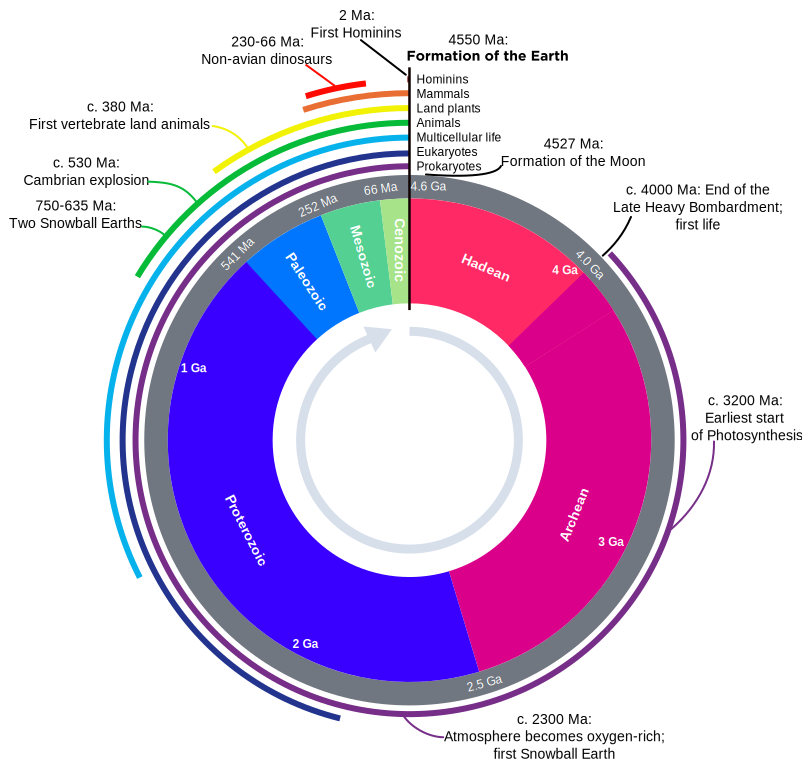
\includegraphics[width=0.7\linewidth]{./figures/appendix1/geologic_clock}

}

\caption{\href{https://commons.wikimedia.org/wiki/File:Geologic_Clock_with_events_and_periods.svg}{Geologic
clock.}}\label{fig:clock}
\end{figure}

\section{Plant Anatomy}\label{plant-anatomy}

\href{https://en.wikipedia.org/wiki/Plant_anatomy}{Plant anatomy} is the
study of the structure of plant cells and tissues, whereas plant
morphology is the study of their external form. All plants are
multicellular eukaryotes, their DNA stored in nuclei. The characteristic
features of plant cells that distinguish them from those of animals and
fungi include a primary cell wall composed of the polysaccharides
cellulose, hemicellulose and pectin, larger vacuoles than in animal
cells and the presence of plastids with unique photosynthetic and
biosynthetic functions as in the chloroplasts. Other plastids contain
storage products such as starch (amyloplasts) or lipids (elaioplasts).

The bodies of vascular plants including clubmosses, ferns and seed
plants (gymnosperms and angiosperms) generally have aerial and
subterranean subsystems. The shoots consist of stems bearing green
photosynthesizing leaves and reproductive structures. The underground
vascularized roots bear root hairs at their tips and generally lack
chlorophyll. Non-vascular plants, the liverworts, hornworts and mosses
do not produce ground-penetrating vascular roots and most of the plant
participates in photosynthesis. The sporophyte generation is
nonphotosynthetic in liverworts but may be able to contribute part of
its energy needs by photosynthesis in mosses and hornworts.

The root system and the shoot system are interdependent -- the usually
nonphotosynthetic root system depends on the shoot system for food, and
the usually photosynthetic shoot system depends on water and minerals
from the root system. Cells in each system are capable of creating cells
of the other and producing adventitious shoots or roots. Stolons and
tubers are examples of shoots that can grow roots. Roots that spread out
close to the surface, such as those of willows, can produce shoots and
ultimately new plants. In the event that one of the systems is lost, the
other can often regrow it. In fact it is possible to grow an entire
plant from a single leaf, as is the case with Saintpaulia, or even a
single cell -- which can dedifferentiate into a callus (a mass of
unspecialized cells) that can grow into a new plant. In vascular plants,
the xylem and phloem are the conductive tissues that transport resources
between shoots and roots. Roots are often adapted to store food such as
sugars or starch, as in sugar beets and carrots.

Stems mainly provide support to the leaves and reproductive structures,
but can store water in succulent plants such as cacti, food as in potato
tubers, or reproduce vegetatively as in the stolons of strawberry plants
or in the process of layering. Leaves gather sunlight and carry out
photosynthesis. Large, flat, flexible, green leaves are called foliage
leaves. Gymnosperms, such as conifers, cycads, Ginkgo, and gnetophytes
are seed-producing plants with open seeds. Angiosperms are
seed-producing plants that produce flowers and have enclosed seeds.
Woody plants, such as azaleas and oaks, undergo a secondary growth phase
resulting in two additional types of tissues: wood (secondary xylem) and
bark (secondary phloem and cork). All gymnosperms and many angiosperms
are woody plants. Some plants reproduce sexually, some asexually, and
some via both means.

\section{Plant Tissues}\label{plant-tissues}

In plant anatomy, tissues are categorized broadly into three tissue
systems:

\begin{enumerate}
\def\labelenumi{\arabic{enumi}.}
\tightlist
\item
  \textbf{Epidermis} - Cells forming the outer surface of the leaves and
  of the young plant body.
\item
  \textbf{Vascular tissue} - The primary components of vascular tissue
  are the xylem and phloem. These transport fluid and nutrients
  internally.
\item
  \textbf{Ground tissue} - Ground tissue is less differentiated than
  other tissues. Ground tissue manufactures nutrients by photosynthesis
  and stores reserve nutrients.
\end{enumerate}

Plant tissues can also be divided differently into two types:

\begin{enumerate}
\def\labelenumi{\arabic{enumi}.}
\tightlist
\item
  \textbf{Meristematic tissue} consists of actively dividing cells, and
  leads to increase in length and thickness of the plant. The primary
  growth of a plant occurs only in certain, specific regions, such as in
  the tips of stems or roots. It is in these regions that meristematic
  tissue is present.
\item
  \textbf{Permanent tissue} is formed when cells from meristematic
  tissues that take up a specific role lose the ability to divide. This
  process of taking up a permanent shape, size and a function is called
  cellular differentiation. Cells of meristematic tissue differentiate
  to form different types of permanent tissue.
\end{enumerate}

There are 3 types of permanent tissues:

\begin{enumerate}
\def\labelenumi{\arabic{enumi}.}
\tightlist
\item
  \textbf{Parenchyma} (para - `beside'; chyma - `in filling, loose,
  unpacked') is the bulk of a substance. In plants, it consists of
  relatively unspecialised living cells with thin cell walls that are
  usually loosely packed so that intercellular spaces are found between
  cells of this tissue. This tissue provides support to plants and also
  stores food. In some situations, a parenchyma contains chlorophyll and
  performs photosynthesis, in which case it is called a chlorenchyma. In
  aquatic plants, large air cavities are present in parenchyma to give
  support to them to float on water. Such a parenchyma type is called
  aerenchyma.
\item
  \textbf{Collenchyma} is Greek word where ``Collen'' means gum and
  ``chyma'' means infusion. It is a living tissue of primary body like
  Parenchyma. Cells are thin-walled but possess thickening of cellulose,
  water and pectin substances (pectocellulose) at the corners where
  number of cells join together. This tissue gives a tensile strength to
  the plant and the cells are compactly arranged and have very little
  inter-cellular spaces. It occurs chiefly in hypodermis of stems and
  leaves. It is absent in monocots and in roots. Collenchymatous tissue
  acts as a supporting tissue in stems of young plants. It provides
  mechanical support, elasticity, and tensile strength to the plant
  body. It helps in manufacturing sugar and storing it as starch. It is
  present in the margin of leaves and resist tearing effect of the wind.
\item
  \textbf{Sclerenchyma} is Greek word where ``Sclrenes'' means hard and
  ``chyma'' means infusion. This tissue consists of thick-walled, dead
  cells. These cells have hard and extremely thick secondary walls due
  to uniform distribution of lignin. Lignin deposition is so thick that
  the cell walls become strong, rigid and impermeable to water.
\end{enumerate}

\section{Coelom}\label{coelom}

The \href{https://en.wikipedia.org/wiki/Coelom}{coelom} is the main body
cavity in most animals and is positioned inside the body to surround and
contain the digestive tract and other organs. The word coelom comes from
Greek: koîlos hollow, cavity. Coelom formation begins in the gastrula
stage. The developing digestive tube of an embryo forms as a blind pouch
called the archenteron.

In Protostomes, the coelom forms by a process known as schizocoely. The
archenteron initially forms, and the mesoderm splits into two layers:
the first attaches to the body wall or ectoderm, forming the parietal
layer and the second surrounds the endoderm or alimentary canal forming
the visceral layer. The space between the parietal layer and the
visceral layer is known as the coelom or body cavity. Examples of
protostome coelomates include earthworms, snails, clams, slugs and
octopuses.

In Deuterostomes, the coelom forms by enterocoely: mesoderm buds from
the walls of the archenteron and hollows to become the coelomic
cavities. Some examples of deuterostome coelomates are sea urchins,
fish, sea stars and humans.

A coelom can absorb shock or provide a hydrostatic skeleton. It can also
support an immune system in the form of coelomocytes that may either be
attached to the wall of the coelom or may float about in it freely. The
fluid inside the coelom is known as coelomic fluid. The coelomic fluid
serves several functions; it acts as a hydroskeleton, it allows free
movement and growth of internal organs, it serves for transport of
gases, nutrients and waste products between different parts of the body,
it allows storage of sperm and eggs during maturation and it acts as a
reservoir for waste.

In the past, some zoologists grouped bilaterian animal phyla based on
characteristics related to the coelom for practical purposes, knowing,
and explicitly stating, that these groups were not phylogenetically
related. Animals were classified in three informal groups according to
the type of body cavity they possess, in a non-taxonomic, utilitarian
way, as the Acoelomata, Pseudocoelomata, and Coelomata. These groups
were never intended to represent related animals, or a sequence of
evolutionary traits.

However, this scheme was followed by a number of college textbooks and
some general classifications, but is now almost totally abandoned as a
formal classification.

\begin{itemize}
\item
  \textbf{Coelomate animals} or Coelomata (also known as eucoelomates
  --- ``true coelom'') have a body cavity called a coelom with a
  complete lining called peritoneum derived from mesoderm (one of the
  three primary tissue layers). The complete mesoderm lining allows
  organs to be attached to each other so that they can be suspended in a
  particular order while still being able to move freely within the
  cavity. Most bilateral animals, including all the vertebrates, are
  coelomates.
\item
  \textbf{Pseudocoelomate animals} have a pseudocoelom (literally
  ``false cavity''), which is a fluid filled body cavity. Tissue derived
  from mesoderm partly lines the fluid filled body cavity of these
  animals. Thus, although organs are held in place loosely, they are not
  as well organized as in a coelomate. All pseudocoelomates are
  protostomes; however, not all protostomes are pseudocoelomates. An
  example of a Pseudocoelomate is the roundworm. Pseudocoelomate animals
  are also referred to as Hemocoel and Blastocoelomate.
\item
  \textbf{Acoelomate animals}, like flatworms, have no body cavity at
  all. Semi-solid mesodermal tissues between the gut and body wall hold
  their organs in place.
\end{itemize}
